\documentclass[11pt]{article}
\usepackage[hidelinks]{hyperref}
\usepackage{graphicx}
\begin{document}

\title{Merck medical papers challenge project documentation}
\author{Maximilian Balthasar Mansky, Richard Schulz}
\date{\today}
\maketitle

\section{Introduction}

The Merck Medical Papers challenge is a public request to develop an algorithm to best predict future citations from a given article. Dataset for this challenge is the open access PubMed bulk package, around 30 GB of medical papers in XML format.

\subsection{Data format}

In the XML format, the data is organised in a tree structure, with meta data and abstract located under \texttt{article/front} and the main text under \texttt{article/body}. The \texttt{article/back} section contains information regarding funding and citations for the body.

Each article file is named with its PMC ID, a unique 7 digit number prefixed by 'PMC', file ending \texttt{.nxml}.

\section{First Steps}

Before delving into the depths of NLP, we first check whether auxiliary information can already predict citations to any accuracy. For this, prepare a table from the files, including the following headers:

\begin{table}[h!]
\begin{tabular}{c c c c}
PMC ID & Journal name & Publication date & Number of citations \\\hline
\texttt{numerical id} & \texttt{string} & \texttt{date} & \texttt{integer}
\end{tabular}
\end{table}

The first three can be extracted from the files, the last one needs to captured from the website. This table will also serve as a master table for connecting citations to PMC ID. Trying to predict the citation count from meta data is not without merit, it has been shown to be highly correlated with the citation count.\footnote{\url{https://github.com/closingsquarebracket/merck_medical_papers}}

Much of the required information is available straight from the index file.\footnote{\url{https://www.ncbi.nlm.nih.gov/pmc/tools/ftp/\#index_files}} From there only the citations need to be retrieved.

An example line from the index file is given here, separated by tabs (\textbackslash t):
\begin{tabular}{c c c c c}
\tiny oa\_package/08/e0/PMC13900.tar.gz & \tiny Breast Cancer Res. 2001 Nov 2; 3(1):55-60 & \tiny PMC13900 & \tiny PMID:11250746 & \tiny NO-CC CODE
\end{tabular}
Explained as location, publication information, PMC and PMID and licence information. Splitting by tabs, the name of the publication and the date can be retrieved by the following regex:
\begin{verbatim}
([\w\s()]+.?)\s(\d{4}\s\w{3}\s\d+);
\end{verbatim}
and for those papers where the day is missing or a month-range is given:
\begin{verbatim}
([\w\s()]+.?)\s(\d{4}\s\w{3})[-;\s]
\end{verbatim}

From here on, the id can be used to match the number of citations through the entrez web interface. After doing so, exploratory data analysis is done through Dataiku's DataScienceStudio. (DSS)
\begin{figure}[h!]
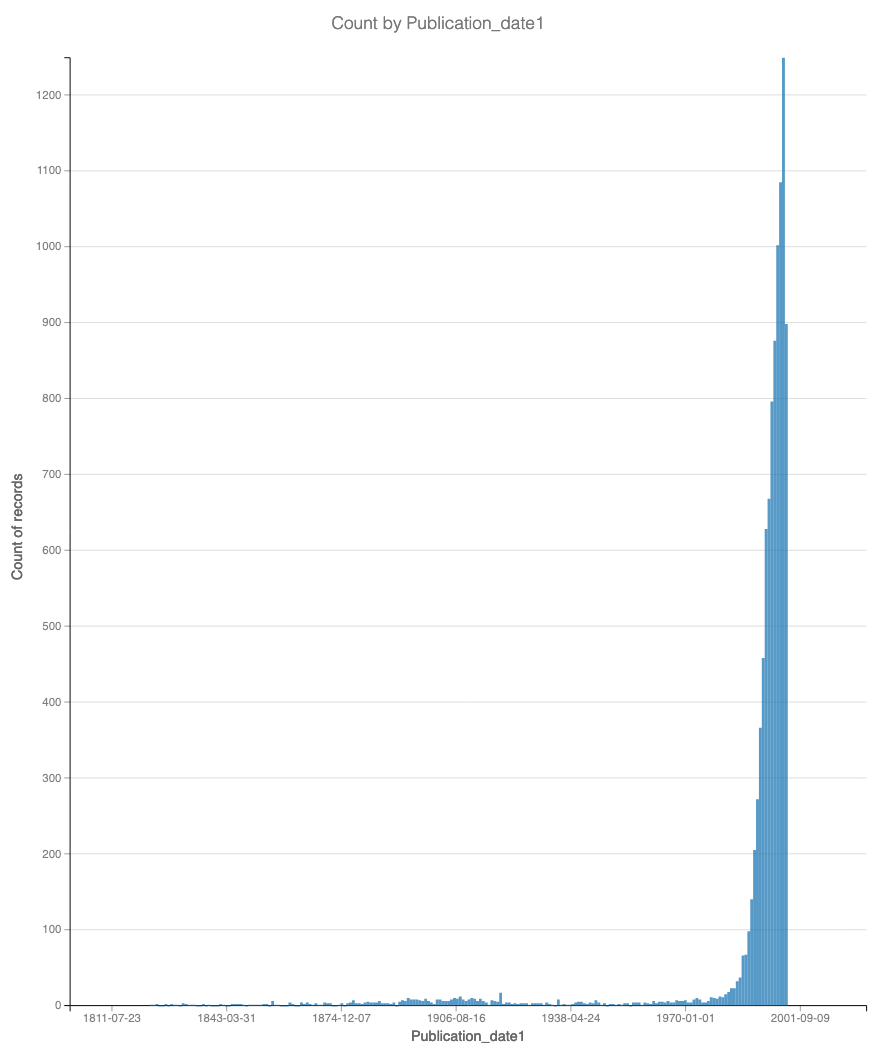
\includegraphics[width=0.48\textwidth]{figures/Count_by_Publication_date1.png}
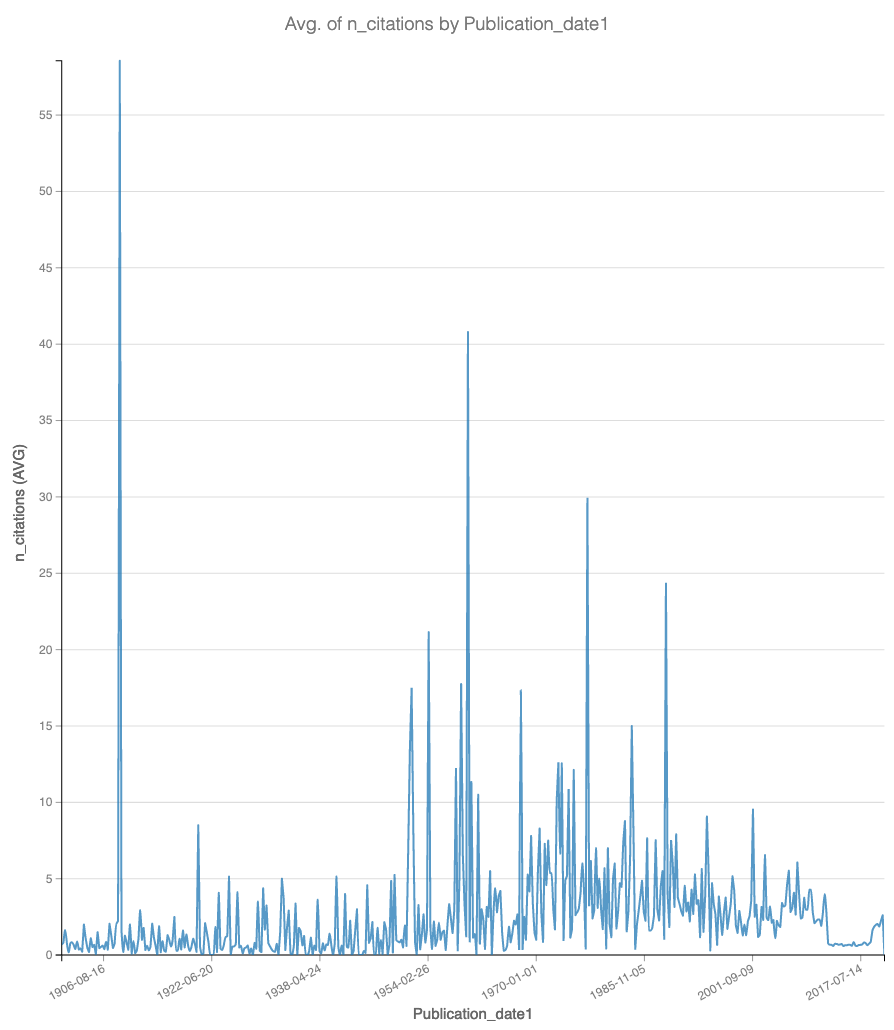
\includegraphics[width=0.48\textwidth]{figures/Avg._of_n_citations_by_Publication_date1.png}
\caption{Timewise distribution of publications and average number of citations over time, for a sample of 10k and 100k random records respectively.}
\end{figure}

It is also possible to run exploratory predictions on the data set, to see whether a pattern is already apparent.

\begin{figure}
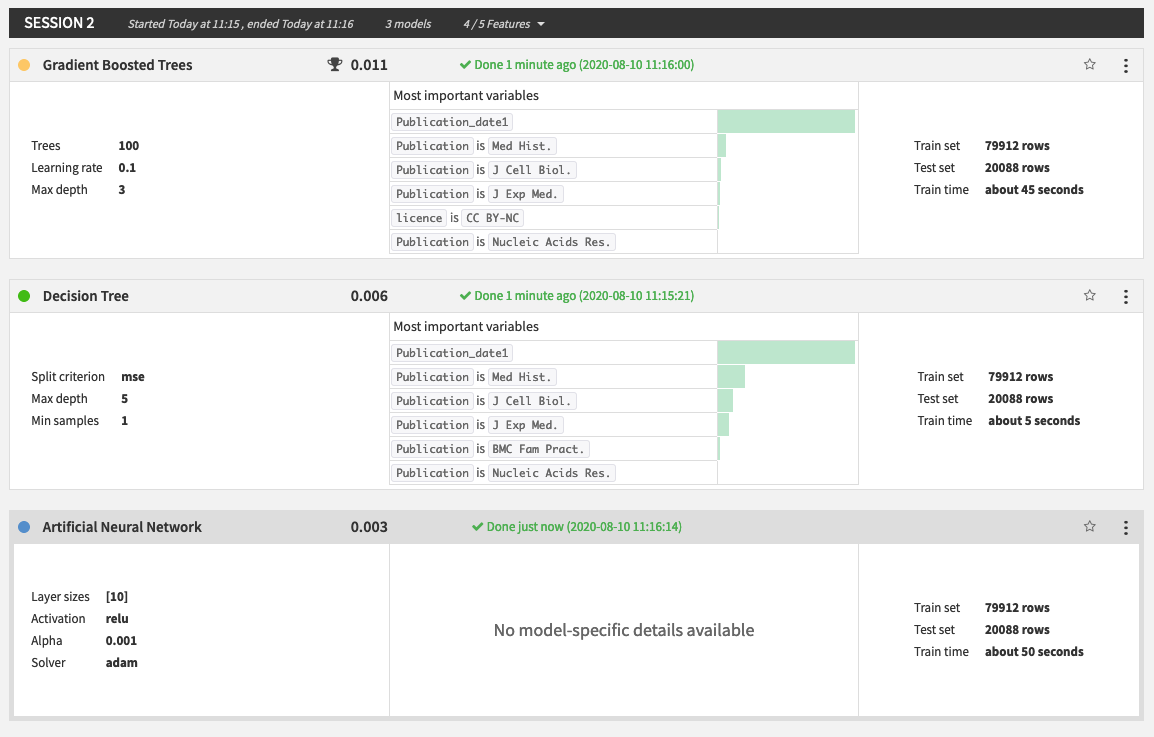
\includegraphics[width=\textwidth]{figures/Quick_search_through_algorithms.png}
\caption{Output screen from DSS, for Gradient Boosted Trees, Decision Tree and Neural Network algorithms.}\label{fig:dss_initial}
\end{figure}

As seen in figure \ref{fig:dss_initial}, no predictions can be made based on the Journal name, publication date and licence alone.\footnote{The PMC ID is ignored, since it is just a unique identifier.} This is to be expected, since a citation should depend on article quality and topic, not on the journal and date alone. For quality, a reasonable indicator can be the author. Most articles are tagged by area, which is included 





\end{document}
